\documentclass[usepdftitle=false, aspectratio=169]{beamer}
\usepackage{pgfpages}

\setbeameroption{hide notes}
\usepackage[theorems]{tcolorbox}

\definecolor{mygreen}{rgb}{.125,.5,.25}

% --- THEME ---
\usetheme[progressbar=frametitle]{metropolis}
\useoutertheme{metropolis}
\useinnertheme{metropolis}
\usefonttheme{metropolis}
\usecolortheme{spruce}  % spruce, metropolis, dove, crane, beaver, seagull
\setbeamercolor{background canvas}{bg=white}
\usecolortheme[named=mygreen]{structure}
\usefonttheme[onlymath]{serif}
\setbeamertemplate{frame numbering}[counter]  % none, counter, fraction

% --- PACKAGES ---
\usepackage[UKenglish]{babel}
\usepackage[utf8]{inputenc}
\usepackage{lmodern}
\usepackage[T1]{fontenc}

% \usepackage{appendixnumberbeamer}
\usepackage{upquote}
\usepackage[straightquotes]{newtxtt}
\usetikzlibrary{positioning}
% \usepackage{minted}
\usepackage{multicol}
\usepackage{xspace}
\usepackage{booktabs}
\usepackage{siunitx}

% --- SETTINGS ---
\graphicspath{{./figures/}}
\setlength{\fboxsep}{0pt}
\frenchspacing
% Avoid font-warning with itemize bullets.
\renewcommand\textbullet{\ensuremath{\bullet}}

% --- OWN COMMANDS ---
\newcommand{\bdra}{\ensuremath{\boldsymbol \Rightarrow }~}
\newcommand{\bdla}{\ensuremath{\boldsymbol \Leftarrow }~}
\newcommand{\dra}{\ensuremath{\Rightarrow }~}
\newcommand{\dla}{\ensuremath{\Leftarrow }~}

\newcommand{\mr}[1]{\mathrm{#1}}

\newcommand{\ohmm}{\ensuremath{\Omega\,}\text{m}\xspace}

\newcommand{\emg}[2]{\texttt{emg#1#2}\xspace}
\newcommand{\empymod}{\texttt{empymod}\xspace}

\newcommand{\rmk}[1]{{\color{red}\bfseries #1}}
\newcommand{\maybe}[1]{{\color{gray} #1}}
\newcommand{\todo}{{\color{red}\texttt{TODO:}}\xspace}
\newcommand{\bm}[1]{{\mathbf{#1}}}

% Add page number to slides
\definecolor{myblue}{rgb}{0,0,.8}
\newcommand{\ato}{\addtocounter{framenumber}{1}}
\newcommand{\code}[1]{\texttt{\color{mygreen}#1}}

% --- TITLE-STUFF ---
\title{Python for Matlab Users}
\subtitle{Computational Seminars @ GSE}
\date{24th June 2024}
\author{Dieter Werthmüller}
\institute{\dra\href{https://github.com/prisae/Python4MatlabUsers}{github.com/prisae/Python4MatlabUsers}}

\hypersetup{
  colorlinks=true,
  urlcolor=myblue,
  citecolor=black,
  filecolor=black,
  linkcolor=black
}

% --- SLIDES ---
\begin{document}
\metroset{block=fill}  % Fills the block-environment
% \usebackgroundtemplate{\includegraphics[width=\paperwidth]{}}

\ato % ---------------------------------------------------------------------- %
\maketitle
% \usebackgroundtemplate{\includegraphics[width=\paperwidth]{}}

% \begin{frame}{Outline} \tableofcontents \end{frame}

% \ato % ---------------------------------------------------------------------- %
% \section{}


\begin{frame}
  {Python for Matlab Users}

  \begin{itemize}\itemsep .6cm
    \item \textbf{What this workshop is}
      \begin{itemize}
        \item A quick primer for Matlab users: What is the same, what is different?
      \end{itemize}
    \item \textbf{What this workshop IS NOT}
      \begin{itemize}
        \item An introduction to programming
        \item An introduction to Python
        \item Best practices and all the other stuff
      \end{itemize}
    \item Ultimate objective of today
      \begin{itemize}
        \item \textbf{YOU start to translate one of your scripts from Matlab to
          Python}
      \end{itemize}
  \end{itemize}
\end{frame}

\begin{frame}
  {Rough comparison}

  \begin{columns}

    \column{.55\textwidth}
    \alert{Python}
    \begin{itemize}
      \item Late 80's (Guido Rossum, then at CWI)
      \item Free and open-source
      \item General programming language;\\
        scientific computing came later (late 90's)
      \item Many ways to install / use
    \end{itemize}

    \column{.45\textwidth}
    \alert{Matlab}
    \begin{itemize}
      \item Late 70's
      \item Proprietary and very costly
      \item Matrix computation
      \item One way to install / use
    \end{itemize}

  \end{columns}

  \vspace{1em}

  Both are multi-paradigm (e.g., \emph{procedural}, \emph{object-oriented}).

  In Python, \emph{everything} is an object.

\end{frame}

\begin{frame}
  {Spyder: \href{https://www.spyder-ide.org}{spyder-ide.org}}
  \dra Easiest for transition, the most “\emph{Matlab-ish}” experience.
  \vspace{1em}

  \begin{columns}
    \column{.4\textwidth}

  \begin{itemize}
    \item Editor with
      \begin{itemize}
        \item cells
        \item linting
        \item visual debugging
      \end{itemize}
    \item Variable explorer
    \item Can run notebooks (\code{spyder-notebook})
    \item Line profiler (\code{spyder-line-profiler})
  \end{itemize}

    \column{.6\textwidth}

    \fbox{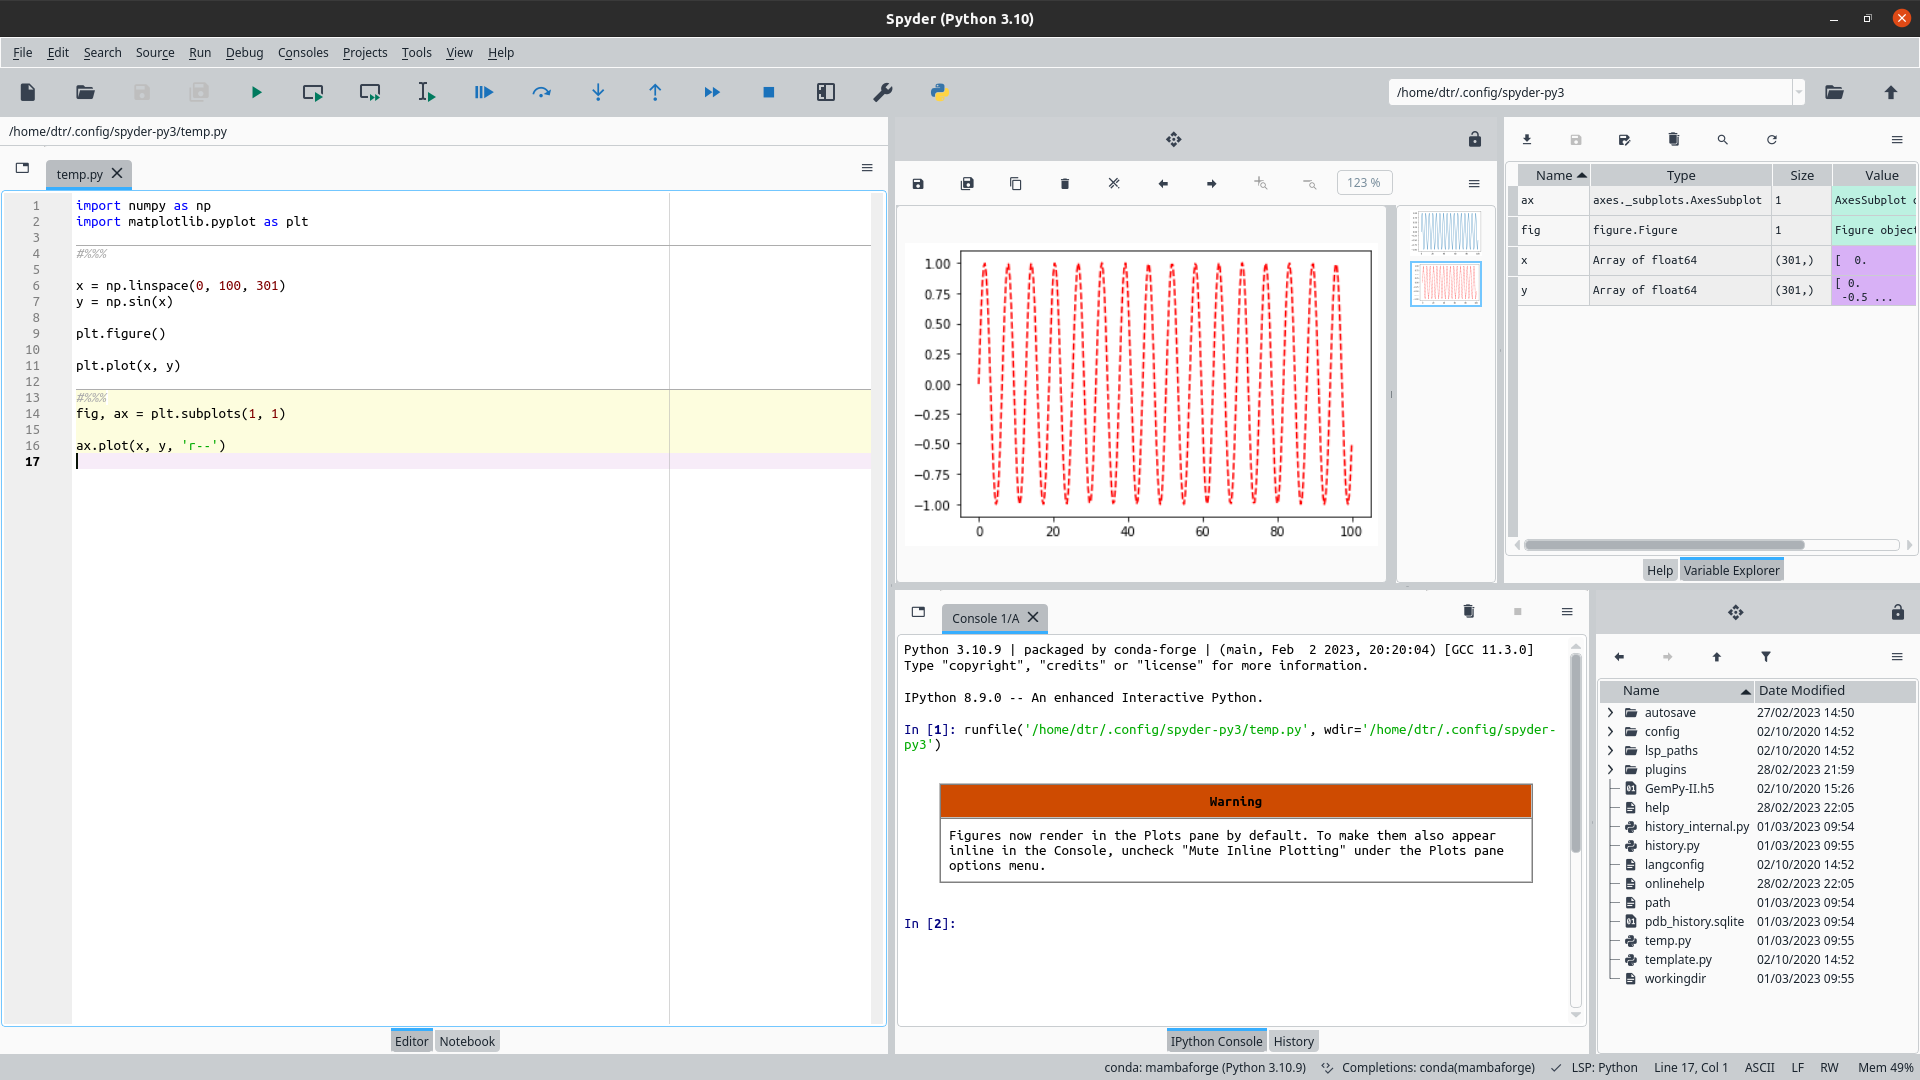
\includegraphics[width=\textwidth]{Spyder}}

  \end{columns}
\end{frame}


\begin{frame}
  {Terminal, Plain Python, IPython (Atom, VSCode, PyCharm, Sublime, \ldots)}


  \begin{columns}
    \column{.5\textwidth}

    Terminal based solutions\\[.2em]
    \fbox{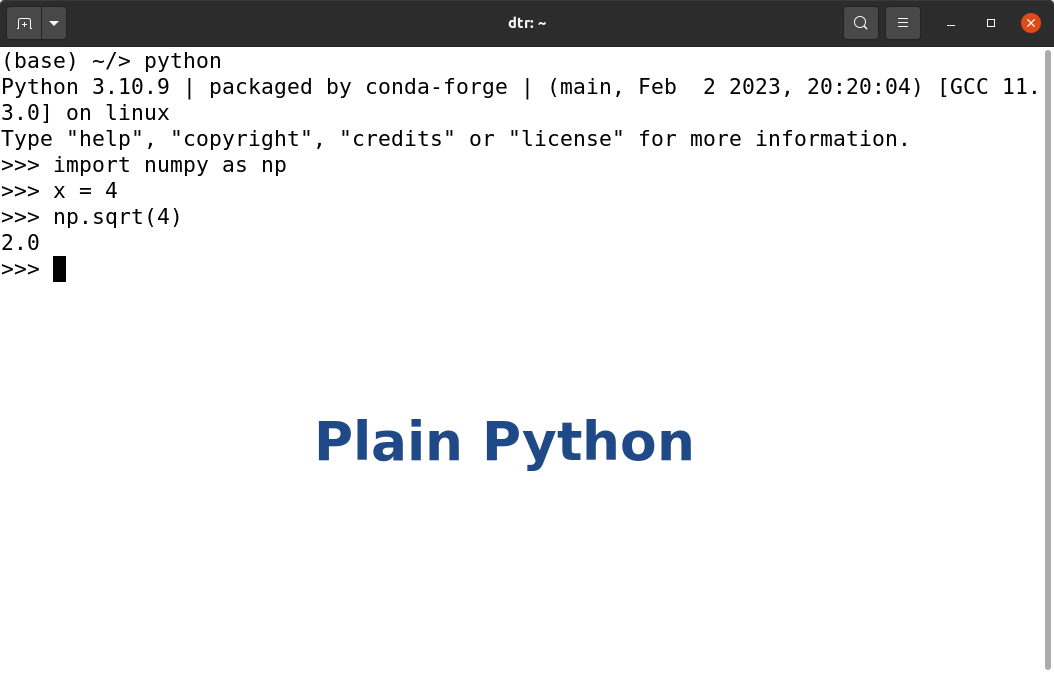
\includegraphics[width=.8\textwidth]{Python}}\\[.2em]
    \fbox{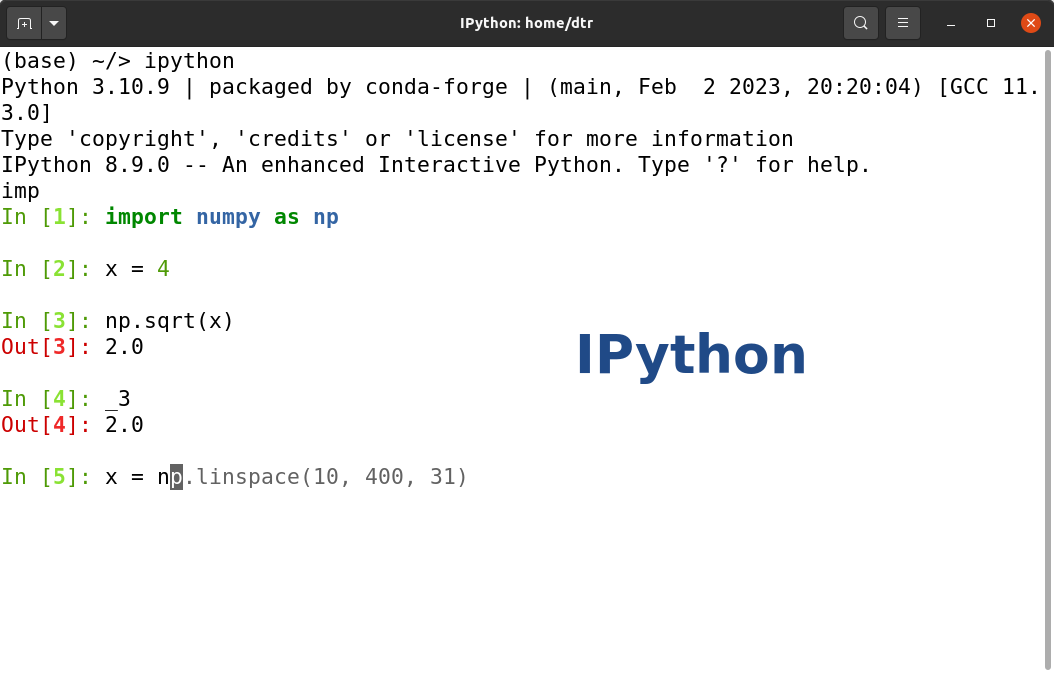
\includegraphics[width=.8\textwidth]{IPython}}

    \column{.5\textwidth}

    Jupyter ecosystem (language agnostic!)\\[.2em]
    \fbox{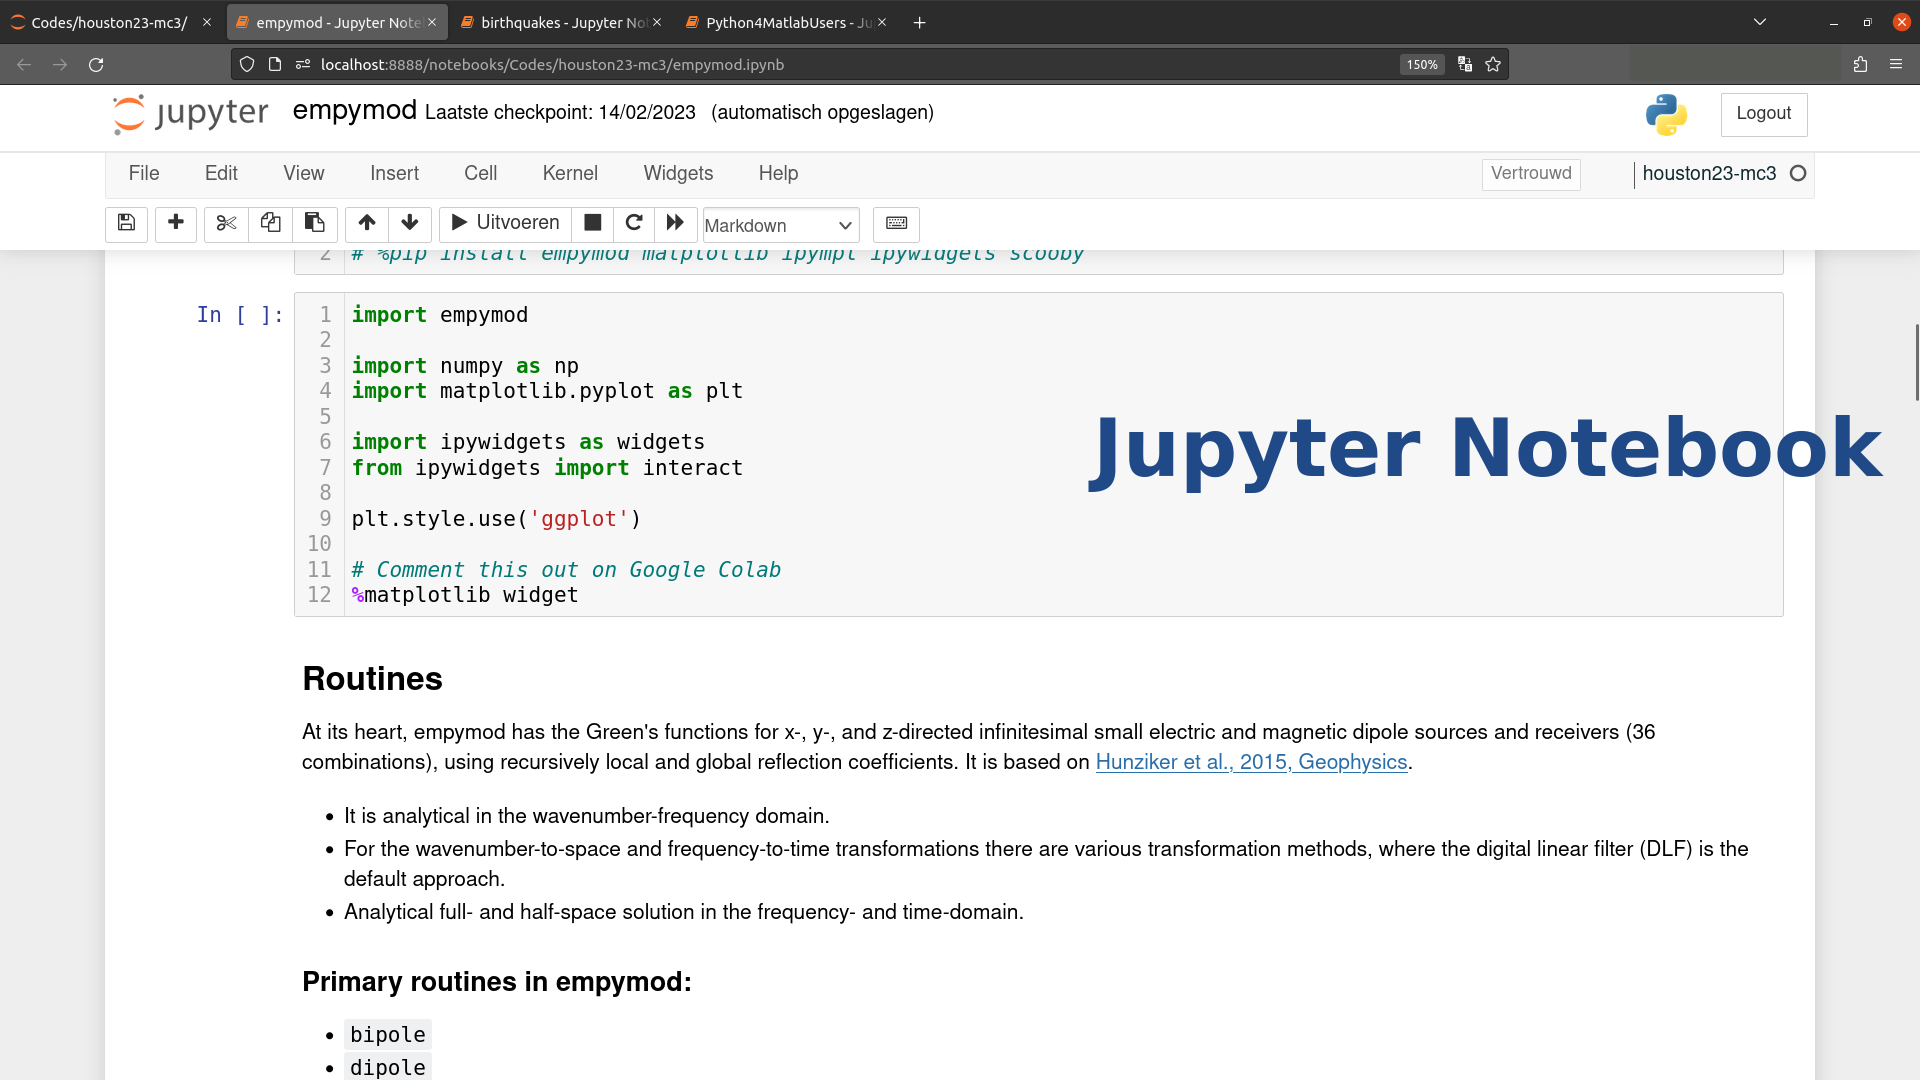
\includegraphics[width=.9\textwidth]{Notebook}}\\[.2em]
    \fbox{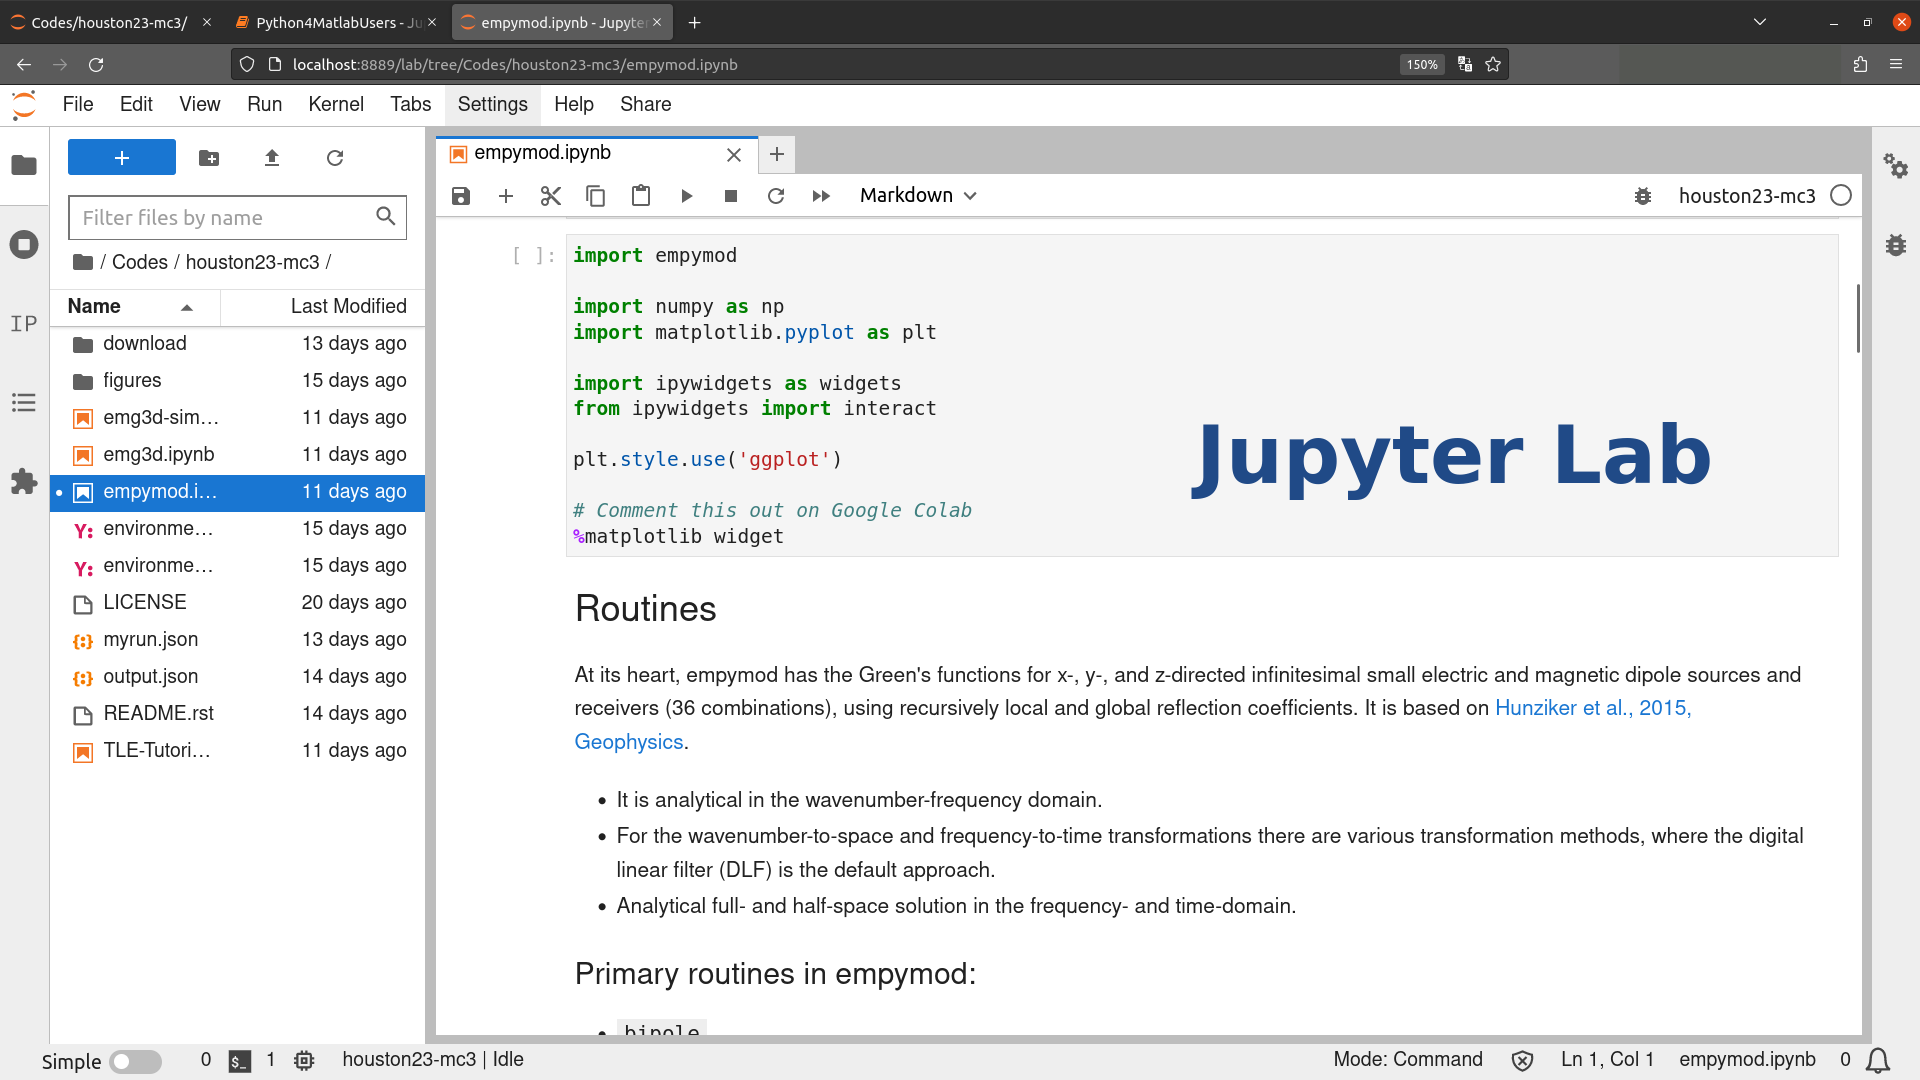
\includegraphics[width=.9\textwidth]{Gitlab}}

  \end{columns}

\end{frame}




\begin{frame}
  {Distributions and Package Manager}

  \begin{columns}
    \column{.5\textwidth}
    \begin{block}{Package Manager}
      \begin{itemize}
        \item \code{pip} (\code{pip install package})
        \item \code{conda} (\code{conda install package})
      \end{itemize}
    \end{block}
    \begin{itemize}
      \item \code{conda} is language agnostic.
    \end{itemize}

    \column{.5\textwidth}
    \begin{block}{Distributions}
      \begin{itemize}
        \item There are many (e.g., Anaconda, conda-forge, Python(x,y); PyPy,
          EDM, WinPython)
        \item I recommend miniforge:
          \href{https://github.com/conda-forge/miniforge}{github.com/conda-forge/miniforge}
      \end{itemize}
    \end{block}

  \end{columns}

  \vspace{1cm}

    Make a note for the future: Once you translated your first scripts, get
    familiar with \textbf{environments}; crucial for \textbf{reproducibility}!
    \href{https://conda.io/projects/conda/en/latest/user-guide/tasks/manage-environments.html}{conda.io/projects/conda/en/latest/user-guide/tasks/manage-environments.html}

\end{frame}

\begin{frame}
  {Why use Python? It is SO SLOW! (I hear it every day)}

  \begin{columns}
    \column{.35\textwidth}
    \begin{itemize}
      \item In scientific computing, \alert{Python is GLUE}
      \item High-level syntax wraps low-level C/Fortran libraries, which is
        (mostly) where the computation happens.
      \item AOT \& JIT: Cython, PyPy, Numba, Pythran, \ldots
    \end{itemize}

    \column{.65\textwidth}
  \fbox{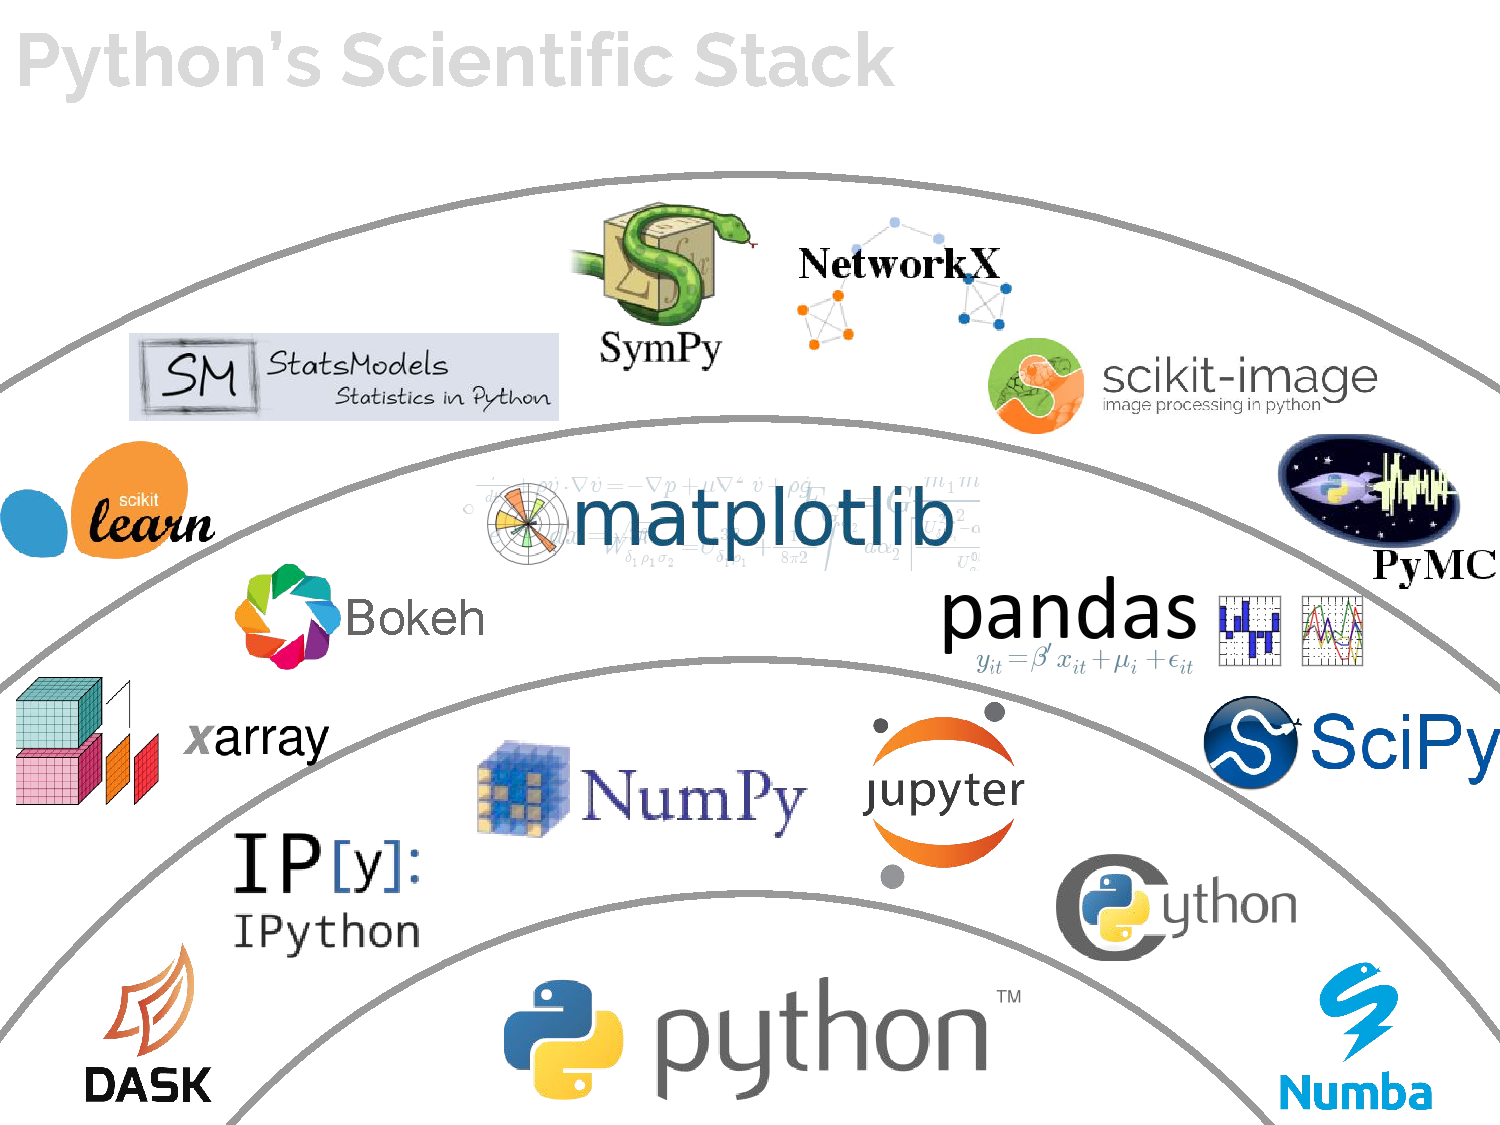
\includegraphics[width=\textwidth]{PyCon_2017-Slide51}}
  \tiny
  \href{https://files.speakerdeck.com/presentations/1083b290db884f2ab5d04eb98580be94/PyCon_2017.pdf}%
  {Jake VanderPlas, PyCon2017, The Unexpected Effectiveness of Python in
  Science}
  \end{columns}

\end{frame}

\begin{frame}
  {Further information}

  \begin{itemize}\itemsep .5cm
    \item \dra Bookmark this:
      \href{https://numpy.org/doc/stable/user/numpy-for-matlab-users.html}%
      {numpy.org/doc/stable/user/numpy-for-matlab-users.html}
    \item More in depth:
      \href{https://www.enthought.com/wp-content/uploads/2019/08/Enthought-MATLAB-to-Python-White-Paper_.pdf}
      {enthought.com/wp-content/uploads/2019/08/Enthought-MATLAB-to-Python-White-Paper\_.pdf}
  \end{itemize}

\end{frame}

% \begin{frame}
%   {Topics not touched}
% 
%   We barely scratch the surface today. This here is a dump-slide for things
%   that come to my mind that we have not talked about.
% 
%   \begin{itemize}
%     \item Duck typing
%     \item \code{global}/\code{local}
%   \end{itemize}
% 
% \end{frame}


\end{document}
